\documentclass[11pt,a4paper]{article}
% \usepackage[utf8]{inputenc}
% \usepackage[T1]{fontenc}
% \usepackage[demo]{graphicx}

\usepackage{algorithm, algorithmicx, algpseudocode} % Algorithm {algorithmic, listings}
\usepackage{amsmath, amstext, amssymb, amsfonts, amsthm, dsfont, cancel, gensymb, mathtools, textcomp} % Math
\usepackage{color, xcolor} % Color
\usepackage{diagbox, multicol, multirow, tabularx} % Table
\usepackage{enumerate} % List
\usepackage{epsfig, epstopdf, graphicx,  palatino, pgfplots, subcaption, tikz, wrapfig} % Image.
\usepackage{cite}
\usepackage{fancybox}
\usepackage{verbatim}

\usepackage[english]{babel}
\usepackage[font=footnotesize]{caption} % labelfont=bf
% \usepackage[font=scriptsize]{subcaption} % labelfont=bf
\usepackage[margin=1in]{geometry}
\usepackage[hidelinks]{hyperref}

\newtheorem{theorem}{Theorem}
\newtheorem{definition}{Definition}
\floatname{algorithm}{Algorithm}
\renewcommand{\algorithmicrequire}{\textbf{Input:}}
\renewcommand{\algorithmicensure}{\textbf{Output:}}
\epstopdfsetup{outdir=./Figure/Converted/}
\graphicspath{{./Figure/}}

\makeatletter
\def\input@path{{./Figure/}}
\makeatother

\newcommand{\image}[3]{
	\begin{figure}[!ht]
		\centering
	    \includegraphics[width=#1\textwidth]{#2}
		\caption{#3}
		\label{fig:#2}
	\end{figure}
}

\title{
	VE475 Introduction to Cryptography\\
	{\Large Lattice-based Cryptography}
}
\author{
	Jiang, Sifan\\
	% jasperrice@sjtu.edu.cn\\
	515370910040
\and
	Wu, Hao\\
	515370910041
\and
	Su, Jingyu\\
	516370910123
\and
	Song, Gaopeng\\
	516370910227
}

\pgfplotsset{compat=1.13}

%%%%% --------------------------------------------------------------------------- %%%%%
\begin{document}
\maketitle
% ------------------------- %
\section{Introduction}
\par A quantum computer is a computer whose operation exploits certain very special transformations of its internal state based on the laws of quantum mechanics and under very carefully controlled conditions \cite{Quantum}. In theory, any particles, like atom, electron, photon, can be used for quantum computing. The reason why quantum computers can have higher computing performance than any regular computers is that one particle can be viewed as a binary $0$, a binary $1$, or a $0$ and $1$ at the same time because of ``Quantum Superposition''. In such way, the computer can conduct parallel computing very efficiently and try all the possible solutions in very short time to realize complex computation. Based on such theory, \textit{Shor} discovered the quantum factoring algorithm with time complexity $O((\log N)^{3})$, making factoring-based cryptosystems no longer secure.
\par New cryptosystems are needed especially nowadays, companies like IBM has developing their own quantum computers, such as \textit{IBM Q System One}. One of the possible post-quantum cryptosystem solution is lattice-based cryptography.
\par Lattices have been introduced to the field of mathematics first in the 18$^{th}$ century in number theory by mathematicians such as Gauss and Lagrange. The study of lattices was advanced by Minkowski in his ``Geometry of Numbers''.
\par In 1982, Arjen Lenstra, Hendrik Lenstra, and L\'{a}szl\'{o} Lov\'{a}sz introduced their famous ``LLL'' basis-reduction algorithm in \textit{Factoring Polynomials with Rational Coefficients} \cite{LLL}, which is used for factoring integer polynomials.
\par In 1996, Mikl\'{o}s Ajtai issued \textit{Generating hard instances of lattice problems} and introduced ``worst-case to average-case reduction'' for lattice problems , providing a cryptographic one-way function based on worst-case hardness conjectures \cite{Ajtai}. And the Short Integer Solution problem (SIS) serve as a foundation of numerous lattice-based cryptographic protocols: For positive integer parameters $n$, $m$, and $q$, find a short non-zero solution $\mathbf{z} \in \mathbb{Z}^{m}$ to the honogeneous linear system $\mathbf{Az} = 0 \mod q$ for uniformly random $\mathbf{A} \in \mathbb{Z}_{q}^{n\times m}$ \cite{LS}. Another main problem, as the foundation, is the Learning With Errors problem.


\subsection{General Lattices}
\par A lattice is a set of points in $n$-dimensional space with a periodic structure , such as the one illustrated in Figure~\ref{fig:2dlattice}, which is a simple example shows the two-dimensional space lattice and two groups of possible, as long as vectors are independent, bases (black and grey ones) \cite{DO}.
\image{0.5}{2dlattice}{A two-dimensional lattice and two possible bases.}
\par Formally, given $n$-independent vectors $\mathbf{b}_{1}, \cdots, \mathbf{b}_{n} \in \mathbb{R}^{n}$, the lattice generated by these vectors is the set of vectors
\begin{align}
	\mathcal{L}(\mathbf{b}_{1}, \cdots, \mathbf{b}_{n}) = \left\lbrace \sum_{i=1}^{n} x_{i}\mathbf{b_{i}} \; : \; x_{i} \in \mathbb{Z} \right\rbrace.
\end{align}
The vectors $\mathbf{b}_{1}, \cdots, \mathbf{b}_{n}$ are known as a basis, denoted $\mathbf{B}$, of the lattice. For example, $\left[1, 5, -9\right]^{T}$, $\left[-2, 2, 0\right]^{T}$, and $\left[13, 1, 4\right]^{T}$ form an basis for $\mathbb{Z}^{3}$ and
\begin{align*}
\mathbf{B} = \begin{bmatrix}
1 & -2 & 13 \\
5 & 2 & 1 \\
-9 & 0 & 4
\end{bmatrix}.
\end{align*}
\par Notice that there exists multiple lattice bases which makes lattice-based cryptography possible. Any lattice can be obtained by applying some non-singular linear transformation to the integer lattice. Also, given $\mathbf{B}_{1}$, $\mathbf{B}_{2}$ two bases for lattice $\mathcal{L}$, there exist uni-modular matrices $\mathbf{U}$ such that $\mathbf{B}_{1} = \mathbf{B}_{2}\mathbf{U}^{-1}$ \cite{DO}.
\par Since lattice is in a periodic structure, the concept of fundamental region is used to formalize this idea. A set $\mathcal{F} \subseteq \mathbb{R}^{n}$ is a fundamental region of a lattice $\mathcal{L}$ if its translates $\mathbf{X} + \mathcal{F} = \{ \mathbf{x} + \mathbf{y} \;:\; y \in \mathcal{F} \}$, taken over all $x \in \mathcal{L}$, form a partition of $\mathbb{R}^{n}$. And the fundamental parallelepiped of a lattice basis $\mathbf{B}$ is defined as
\begin{align}
	\mathcal{P}(\mathbf{B}) := \mathbf{B} \cdot \left[ -\frac{1}{2}, \frac{1}{2} \right)^{n} = \left\lbrace \sum_{i=1}^{n} c_{i}\mathbf{b}_{i} \;:\; c_{i} \in \left[ -\frac{1}{2}, \frac{1}{2} \right) \right\rbrace.
\end{align}
\par Then, the determinant of a lattice $\mathcal{L}$, denoted $\det(\mathcal{L})$, can be defined as $\mathrm{vol}(\mathcal{F})$.
\par Since a lattice $\mathcal{L}$ is discrete, it has two non-zero elements $\pm \mathbf{v} \in \mathcal{L}$ of minimum Euclidean distance. The exact definition of the minimum distance of a lattice $\mathcal{L}$ is defined as
\begin{align}
\lambda_{1}(\mathcal{L}) := \min_{\mathbf{v}\in\mathcal{L}\setminus\left\lbrace\mathbf{0}\right\rbrace} \|\mathbf{v}\|.
\end{align}
\par With Minkowski's First Theorem, we have for any lattice $\mathcal{L}$, we have $\lambda_{1}(\mathcal{L}) \leq \sqrt{n}\cdot\det(\mathcal{L})^{1/n}$. And using the exact formula for the volume of an $n$-dimensional ball, we can obtain a slightly tiger bound $\lambda_{1}(\mathcal{L}) \leq \sqrt{n/(2\pi e)}\cdot\det(\mathcal{L})^{1/n}$.


\subsection{Lattice Problems}
\subsubsection{Shortest Vector Problem}
\par Shortest Vector Problem (SVP) is the most important lattice-based computational problem, which requires the approximate of the minimal Euclidean length of a non-zero lattice vector. The definition of Approximated Shortest Vector Problem (SVP$_{\gamma}$) is: find a vector $\mathbf{v} \in \mathcal{L}(\mathbf{B}) \setminus \{\mathbf{0}\}$ such that
\begin{align*}
\|\mathbf{v}\| \leq \gamma \cdot \min_{\mathbf{w} \in \mathcal{L}(\mathbf{B})\setminus\mathbf{0}}  \|\mathbf{w}\|
\end{align*}
\par Where $\gamma \geq$ and when $\gamma = 1$, it's a non-approximated problem. There are three common variants of SVP \cite{Peikert}:
\begin{enumerate}
\item Decision (GapSVP$_{\gamma}$): given a lattice basis $\mathbf{B}$ and a positive integer $d$, distinguish between the cases $\lambda_{1}(\mathcal{L}(\mathbf{B})) \leq d$ and $\lambda_{1}(\mathcal{L}(\mathbf{B})) > \gamma \cdot d$.
\item Estimate (EstSVP$_{\gamma}$): given a lattice basis $\mathbf{B}$, compute $\lambda_{1}(\mathcal{L}(\mathbf{B}))$ up to a $\gamma$ factor, i.e., output some $d \in [\lambda_{1}(\mathcal{L}(\mathbf{B})), \gamma \cdot \lambda_{1}(\mathcal{L}(\mathbf{B}))]$.
\item Search: with is SVP$_{\gamma}$ itself.
\end{enumerate}
\par To efficiently compute bounds on the minimum distance, and even find relatively short non-zero lattice vectors, Lenstra-Lenstra-Lov\'{a}sz (LLL) algorithm can be applied. It yields a polynomial-time solution to SVP$_{\gamma}$  with an approximation factor $\gamma = 2^{n-1}-2$, which is exponential in the dimension. It ``converts an arbitrary lattice into one that generates the same lattice, and which is “reduced” in the following sense''\cite{Peikert}.

\subsubsection{Shortest Independent Vectors Problem}
\par Approximated Shortest Independent Vector Problem (SIVP$_{\gamma}$) is: find $\mathbf{U}\in \mathrm{Gl}_{n}(\mathbb{Z})$ with
\begin{align*}
\|\mathbf{B}\mathbf{U}\| \leq \gamma \cdot \min_{\mathbf{V}\in \mathrm{Gl}_{n}(\mathbb{Z})} \|\mathbf{B}\mathbf{V}\|
\end{align*}

\subsubsection{Closet Vector Problem}
\par Approximated Closet Vector Problem (CVP$_{\gamma}$) is: for $\mathbf{t} \in \mathbb{R}^{n}$, find a lattice point $\mathbf{v}\in \mathcal{L}(\mathbf{B})$ such that
\begin{align*}
\| \mathbf{v} - \mathbf{t}\| \leq \gamma \cdot \min_{\mathbf{w}\in \mathcal{L}(\mathbf{B})} \|\mathbf{w} - \mathbf{t}\|
\end{align*}
\section{GGH/HNF \cite{JL}}
Though The GGH/HNF cryptosystem, proposed by Goldreich, Goldwasser and Halevi has already been broken in practice, it's still valuable to learn it while studying lattice based cryptography.

\subsection{Related Knowledge}
For any $n \times m$ matrices $A \in \mathbb{Z}^{n \times m}$ with rank m, there exists a uni-modular matrix $U$(i.e. $\det(U)=\pm1$) such that 
$$
UA = H, 
$$
where $h_{ii}$ is positive for $1\leq i\leq m$, $h_{ij}=0$ for $j>i$, and $\left|h_{ij}\right|<h_{ii}$ for $i>j$  \cite{MSKNA}. $H$ is called the Hermite normal form  of A.

\subsection{Key Generation}
For a chosen lattice base $B$, we can calculate its Hermite Normal Form $H$ by finding a uni-modular matrix $U$(i.e. $\det(U)=\pm1$) and 
$$H=BU.$$
Then $B$ is the private key and $H$ is the public key.


\subsection{Encryption}
If the message is $m \in \mathbb{Z}^n$, then the ciphertext $c \in \mathbb{Q}^n$ is 
$$
c=Hm+r,
$$
where $r \in \mathbb{Q}^n $ is a small noise vector chosen such that the lattice vector closest to c is $Hm$.


\subsection{Decryption}
For the ciphertext message $c \in \mathbb{Q}^n$, the private key $B$ and the public key $H=BU$, first compute:
$$
B^{-1} \cdot c =B^{-1} \cdot (Hm + r) = B^{-1}BUm + B^{-1}r = Um + B^{-1}r.
$$
Then since r is a small noise by definition, use the babai rounding method\cite{BL}  to remove the term $B^{-1}r$. Finally get m by $$U^{-1}Um=m$$
\section{The LWE-based cryptosystem}

\subsection{Introduction}

The LWE-based cryptosystem is proved to be the most efficient lattice-based cryptosystem to date which is supported by a theoretical proof of security. The cryptosystem is shown to be secure based on the conjectured hardness of the \textbf{L}earning \textbf{W}ith \textbf{E}rrors problem (LWE), where the definition is shown below.

\begin{algorithm}
    \caption{Learning-With-Errors (LWE)}
    \begin{algorithmic}
        \State \textit{Parameters}: Integers $n, m, q \in \mathbb{Z}_{+}$ and a probability distribution $\chi : \mathbb{Z}_{q} \rightarrow[0,1]$.
        \State \textit{Instance}: A pair $(A, v)$ with $A \in \mathbb{Z}_{q}^{m \times n}$ and $v \in \mathbb{Z}_{q}^{m}$.
        \State \textit{Problem Task}: Decide if $v \in_{R} \mathbb{Z}_{q}^{m}$ was chosen uniformly at random or $v=A s+e$ was chosen with $s \in _R \mathbb{Z}_{q}^{n}$ and $e \in_{\chi} \mathbb{Z}_{q}^{m}$.
    \end{algorithmic}
\end{algorithm}

This problem can be equivalently described as a bounded distance decoding problem in $q$-ary lattices: Given $A \in_{R} \mathbb{Z}_{q}^{m \times n}$ and a vector $v \in \mathbb{Z}_{q}^{m},$ we need to distinguish between the case that $v$ is chosen uniformly from $\mathbb{Z}_{q}^{m}$ and the case in which $v$ is chosen by mangling each coordinate of a random point in $\Lambda_{q}\left(A^{T}\right)$ using $\chi^{m}.$

The LWE problem is believed to be very hard (for reasonable choices of parameters), with the best known algorithms running in exponential time in $n$. For a real $\alpha>0$ we let $\chi=\Psi_{\alpha}$ denote the distribution on $\mathbb{Z}_{q}$ obtained by sampling a normal variable with mean 0 and standard deviation $\alpha q / \sqrt{2 \pi}$ , rounding the result to the nearest integer and reducing it modulo $q$. Furthermore, we have the following theorem proven.

\begin{theorem}
    Assume access to an oracle that solves the LWE problem with a parameter choice $(n, m, q, \chi)$ such that $\chi=\Psi_{\alpha},\ \alpha q>\sqrt{n},$ a prime $q \leq \operatorname{poly}(n)$ and $m \leq \operatorname{poly}(n) .$ Then, there exists a quantum algorithm running in time poly $(n)$ for solving the SIVP$_{\gamma}$ and the decision variant of SVP$_{\gamma}$ for $\gamma=\tilde{\mathcal{O}}(n / \alpha)$ in any lattice of dimension $n$.\label{the1}
\end{theorem}

In other words, when we consider the security of lattice-based problems against quantum computers, any cryptosystem based on LWE is also secure against quantum computers. Moreover, it is very much possible that the proof for Theorem \ref{the1} may some day be dequantized, i.e. ported to a classical computational model, leading to a stronger security guarantee for LWE-based cryptosystems. Also, it has to be emphasized that the quantum arguments only show up in the LWE problem itself, and all of the cryptosystems based on it are entirely classical.

\subsection{Cryptosystem}

\subsubsection{Key Generation}

The cryptosystem is parameterized by integers $n, m, \ell, t, r, q,$ and a real $\alpha>0$. The parameter $n$ is in some sense the main security parameter, and it corresponds to the dimension of the lattices that show up in the worst-case connection. The generation pattern of both the public key and the private key is shown below.

\begin{algorithm}
    \caption{LWE-Key-Generation}
    \begin{algorithmic}[1]
        \Require $n, m, \ell, t, r, q \in \mathbb{Z}_{+}$ and $\alpha \in \mathbb{R}_{+}$
        \Ensure private key $S \in \mathbb{Z}_{q}^{n \times \ell}$ and public key $(A, P) \in \mathbb{Z}_{q}^{m \times n} \times \mathbb{Z}_{q}^{m \times \ell}$
        \State \textbf{choose} $S \in_{R} \mathbb{Z}_{q}^{n \times \ell}, A \in_{R} \mathbb{Z}_{q}^{m \times n}, E \in \Psi_{\alpha} \mathbb{Z}_{q}^{m \times \ell}$
        \State \textbf{set} $P :=A S+E$
        \State \Return $(S,(A, P))$
    \end{algorithmic}
\end{algorithm}

\subsubsection{Encryption}

To better understand the encryption algorithm, the following definition is needed.

\begin{definition}
    For integers $q, t \in \mathbb{Z}_{+},$ we define a function $\rho_{t}^{q} : \mathbb{Z}_{t} \rightarrow \mathbb{Z}_{q}$ by $$\rho_{t}^{q}(n) :=\left[\frac{n q}{t}\right].$$ We also write $\rho_{t}^{q}$ instead of $\left(\rho_{t}^{q}\right)^{\ell}$ when we apply this function to vectors in $\mathbb{Z}_{t}^{\ell}$.\label{def1}
\end{definition}

The encryption algorithm is shown below.

\begin{algorithm}
    \caption{LWE-Encryption}
    \begin{algorithmic}[1]
        \Require $n, m, \ell, t, r, q \in \mathbb{Z}_{+}, \alpha \in \mathbb{R}_{+},$ public key $(A, P) \in \mathbb{Z}_{q}^{m \times n} \times \mathbb{Z}_{q}^{m \times \ell},$ message $v \in \mathbb{Z}_{t}^{\ell}$
        \Ensure ciphertext $(u, c) \in \mathbb{Z}_{q}^{n} \times \mathbb{Z}_{q}^{\ell}$
        \State \textbf{choose} $a \in R[-r, r]^{m} \cap \mathbb{Z}^{m}$
        \State \textbf{set} $u :=A^{T} a$
        \State \textbf{set} $c :=P^{T} a+\rho_{t}^{q}(v)$
        \State \Return $(u,c)$
    \end{algorithmic}
\end{algorithm}

\subsubsection{Decryption}

The decryption algorithm is shown below. Also, to make the complete cryptosystem more intuitive, a schematic diagram is illustrated in Figure \ref{fig1} shown below as well.

\begin{algorithm}
    \caption{LWE-Decryption}
    \begin{algorithmic}[1]
        \Require ciphertext $(u, c) \in \mathbb{Z}_{q}^{n} \times \mathbb{Z}_{q}^{\ell},$ private key $S \in \mathbb{Z}_{q}^{n \times \ell}$
        \Ensure $v \in \mathbb{Z}_{t}^{\ell}$
        \State \Return $\rho_{q}^{t}\left(c-S^{T} u\right)$
    \end{algorithmic}
\end{algorithm}

\begin{figure}[htbp]
    \centering
    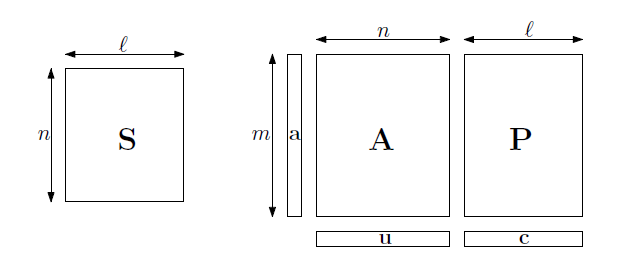
\includegraphics[height=5.0cm]{Figure/sgp1.png}}
    \caption{Ingredients in the LWE-based cryptosystem.}
    \label{fig1}
\end{figure}

\subsection{Choosing Parameters}

The choice of parameters is meant to guarantee efficiency, a low probability of decryption errors, and security. In the following sections we will discuss how to choose the parameters in detail covering all these aspects.

\subsubsection{Efficiency}

The cryptosystem can be implemented efficiently since the operations only involve matrix addition and multiplication modulo a certain integer. Because of the features of computers, it is obvious to set $t=2^k$ to improve the running time. Also, the algorithms can be implemented with high level of parallelization, which is also easy to obtain.

\subsubsection{Decryption Errors}

Let $b :=E^{T} a$ and assume $\left|b_{i}\right|<\frac{q}{2 t}-\frac{1}{2} .$ We also set $w :=\rho_{t}^{q}(v),$ so we know
$$\left|\frac{q v_{i}}{t}-w_{i}\right| \leq \frac{1}{2} \Leftrightarrow\left|v_{i}-\frac{t w_{i}}{q}\right| \leq \frac{t}{2 q}$$

We now get 
$$\rho_{q}^{t}\left(b_{i}+\rho_{t}^{q}\left(v_{i}\right)\right)=\left[\frac{t \cdot\left(b_{i}+w_{i}\right)}{q}\right]$$

Therefore, we can calculate the estimate as
\begin{equation}
    \left|v_{i}-\frac{t \cdot\left(b_{i}+w_{i}\right)}{q}\right|=\left|v_{i}-\frac{t w}{q}\right|+\left|\frac{t b_{i}}{q}\right|<\frac{t}{2 q}+\left(\frac{1}{2}-\frac{t}{2 q}\right)=\frac{1}{2}\label{eq1}
\end{equation}

Thus, we can get 
\begin{align*}
    \rho_{q}^{t}\left(c-S^{T} u\right)&=\rho_{q}^{t}\left(P^{T} a+\rho_{t}^{q}(v)-S^{T} A^{T} a\right)\\
    &=\rho_{q}^{t}\left((A S+E)^{T} \cdot a+\rho_{t}^{q}(v)-S^{T} A^{T} a\right)\\
    &=\rho_{q}^{t}\left(E^{T} a+\rho_{t}^{q}(v)\right) \stackrel{(\ref{eq1})}{=} v
\end{align*}

Since $q$ is odd, if we assume $t$ to be even, we can conclude that
$$\left|b_{i}\right|<\frac{q}{2 t}-\frac{1}{2} \Leftrightarrow t\left|b_{i}\right|<\frac{q-t}{2} \Leftrightarrow t\left|b_{i}\right|<\frac{q}{2} \Leftrightarrow\left|b_{i}\right|<\frac{q}{2 t}$$

In other words, under this assumption, we can get
\begin{equation}
    \operatorname{Pr}\left[\rho_{q}^{t}\left(c-S^{T} u\right)=v\right] \geq \operatorname{Pr}\left[\forall i :\left|b_{i}\right|<\frac{q}{2 t}\right]\label{eq2}
\end{equation}

Now we analyze the behaviour of $b=E^{T} a$. Since each coordinate of $a$ is uniformly chosen from $[-r, r] \cap \mathbb{Z}$, we can get the variance of each coordinate
$$\operatorname{Var}\left(a_{i}\right)=\frac{1}{2 r+1} \cdot \sum_{k=-r} k^{2}=\frac{1}{2 r+1} \cdot \frac{r \cdot(r+1) \cdot(2 r+1)}{6}=\frac{r(r+1)}{3}$$

We denote by $X$ the random variable measuring $b_{i}$ and by $Z :=\frac{X-\mu(X)}{\sigma(X)}$ its normalization, such that $\operatorname{Pr}\left[z_{1} \leq Z \leq z_{2}\right]=\phi\left(z_{2}\right)-\phi\left(z_{1}\right) .$ Thus, we can calculate
    $$\sigma(X)^{2}=\operatorname{Var}\left(b_{i}\right)=\operatorname{Var}\left(\sum_{j=1}^{m} E_{j i} a_{j}\right)=\sum_{j=1}^{m} \operatorname{Var}\left(E_{j i}\right) \cdot \operatorname{Var}\left(a_{j}\right)=m \cdot \frac{\alpha^{2} q^{2}}{2 \pi} \cdot \frac{r(r+1)}{3}$$
and deduce an upper bound for the decryption error probability per letter:
\begin{align*}
    \operatorname{Pr}\left[|X| \geq \frac{q}{2 t}\right]&=\operatorname{Pr}\left[Z \geq \frac{q}{2 t \sigma(X)}\right]+\operatorname{Pr}\left[Z \leq \frac{-q}{2 t \sigma(X)}\right]\\
    &=1-\phi\left(\frac{q}{2 t \sigma(X)}\right)+\phi\left(\frac{-q}{2 t \sigma(X)}\right)\\
    &=2-2 \cdot \phi\left(\frac{q}{2 t \cdot \sigma(X)}\right)\\
    &=2 \cdot\left(1-\phi\left(\frac{1}{2 t \alpha} \cdot \sqrt{\frac{6 \pi}{r \cdot(r+1) \cdot m}}\right)\right)
\end{align*}

Plug into (\ref{eq2}), we can obtain
$$\operatorname{Pr}\left[\rho_{q}^{t}\left(c-S^{T} u\right) \neq v\right]<\operatorname{Pr}\left[\forall i :\left|b_{i}\right| \geq \frac{q}{2 t}\right]=1-\left(1-\operatorname{Pr}\left[\exists i :\left|b_{i}\right| \geq \frac{q}{2 t}\right]\right)^{\ell}$$

Then, the problem is deduced to mere arithmetics to adjust parameters accordingly to obtain low error margins. With some efforts, we can get the error-correcting codes to the plaintext to reduce the probability of decoding errors to a certain small value, which can be neglected.

\subsubsection{Security}

To meet the requirements of Theorem \ref{the1}, we choose $q$ to be prime and $\alpha q>\sqrt{n}$. This leaves us with a choice for $m$ and $\alpha$ where we will attempt to choose $\alpha$ as large as possible since it leads to harder lattice instances. Under these conditions, we may assume that the public keys are completely indistinguishable from pairs $(A, P)$ which is chosen uniformly at random. 

Despite all these theoretical results, we would like to describe an attack that is the best among all to break the cryptosystem. Assume that $(A, v)$ is an LWE-instance.

\begin{itemize}
    \item Choose a short vector $w \in \Lambda_{q}\left(A^{T}\right)^{*}$
    \item Calculate $\lambda :=\langle w, v\rangle$
    \item If $\lambda$ is close to an integer, we guess that $v=A s+e$ for some $e \in \Psi_{\alpha} \mathbb{Z}_{q}^{m}$
\end{itemize}

This method is based on the fact that 
$$\langle A s+e, w\rangle=\underbrace{\langle A s, w\rangle}_{\in \mathbb{Z}}+\langle e, w\rangle$$
and relies on $\langle e, w\rangle$ being very small. Fixing any vector $w$ and for $e \in \Psi_{\alpha} \mathbb{Z}_{q}^{m}$,
$$\operatorname{Var}(\langle e, w\rangle)=\operatorname{Var}\left(\sum_{i=1}^{m} e_{i} w_{i}\right)=\sum_{i=1}^{m} w_{i}^{2} \operatorname{Var}\left(e_{i}\right)=\|a\|^{2} \cdot \frac{\alpha^{2} q^{2}}{2 \pi}$$
yields a standard deviation of $\|w\| \cdot \frac{\alpha q}{\sqrt{2 \pi}}$ for this value. Since we want the above algorithm to fail, we choose
\begin{equation}
    \frac{\alpha q}{\sqrt{2 \pi}} \gg \frac{1}{\|w\|}\label{eq3}
\end{equation}

Based on the lattice reduction method, we have 
$$\Lambda_{q}\left(A^{T}\right)^{*}=q^{-1} \Lambda_{q}^{\perp}\left(A^{T}\right)$$
which result in
$$\|w\| \approx q^{-1} \cdot \min \left(q, 2^{\sqrt{4 n \log (q) \log (\delta)}}\right)$$

If right and left hand side of (\ref{eq3}) differ by a factor of $1.5,$ this brings the distribution of $\lambda$ mod $\mathbb{Z}$ into negligible statistical distance from the uniform distribution. Then, we get 
\begin{equation}
    \alpha \geq 1.5 \cdot \sqrt{2 \pi} \max \left(q^{-1}, 2^{-2} \sqrt{n \log (q) \log (\delta)}\right)\label{eq4}
\end{equation}

For a pair $(A, P) \in_{R} \mathbb{Z}_{q}^{m \times n} \times \mathbb{Z}_{q}^{m \times \ell}$ chosen uniformly at random and used as a public key for LWE-Encryption, we would like the ciphertext to be indistinguishable from a uniformly chosen vector. This would establish the cryptosystem extremely secure against chosen plaintext attacks.

\begin{theorem}
    Let $r<q$ be integers, $M \in R \mathbb{Z}_{q}^{n \times m}$ and $a \in R[-r, r]^{m} \cap \mathbb{Z}_{q}^{m} .$ Then, the statistical distance between the distribution of $M a$ and the uniform distribution on $\mathbb{Z}_{q}^{n}$ is bounded by $$\beta_{n, m}(q, r) :=\sqrt{\frac{(2 r+1)^{m}}{q^{n}}}$$\label{the2}
\end{theorem}

Choosing $M=\left(\begin{array}{c}{A^{T}} \\ {P T}\end{array}\right),$ Theorem \ref{the2} suggest we should choose parameters in such a way that $\beta_{n+\ell, m}(q, r)$ is negligible, which, in other words, $\beta_{n+\ell, m}(q, r)=2^{-100}$.

\subsubsection{Summary}

In this summary, we present some concrete choices of parameters, satisfying our aforementioned requirements. Thus, we expect them to deliver high levels of both security and efficiency. Equation (\ref{eq3}) result in the following choice:
$$m :=\frac{(n+\ell) \log (q)+200}{\log (2 r+1)}$$

Using an approximation parameter of $\delta=1.01$ corresponds to the most exact algorithm known, thus the estimate (\ref{eq4}) result in a choice of
$$\alpha :=4 \cdot \max \left\{q^{-1}, 2^{-2 \sqrt{n \log (q) \log (1.01)}}\right\}$$

We then can list some properties for the cryptosystem, which are quite intuitive and easy to observe, or otherwise ease to be derived from the above listed equations. The sizes are all in bits, and the logarithms are base 2.

\begin{itemize}
    \item Private key size: $n \ell \log q$
    \item Public key size: $m(n+\ell) \log q$
    \item Message size: $\ell \log t$
    \item Ciphertext size: $(n+\ell) \log q$
    \item Encryption blowup factor: $\left(1+\frac{n}{\ell}\right) \log q / \log t$
    \item Error probability per letter: $2 \cdot\left(1-\phi\left(\frac{1}{2 t \alpha} \cdot \sqrt{\frac{6 \pi}{r \cdot(r+1) \cdot m}}\right)\right)$
    \item Lattice dimension in attack: $\sqrt{n \log (q) / \log (\delta)}$
\end{itemize}

\begin{table}[!ht]
    \centering
    \begin{tabular}{|c||c|c|c|c|c|c|}
        \hline
        $n$ &136 &166& 192& 214& 233& 233\\\hline
        $l$ &136& 166& 192& 214& 233& 233\\\hline
        $m$ &2008& 1319& 1500& 1333& 1042& 4536\\\hline
        $q$ &2003& 4093& 8191& 16381& 32749& 32749\\\hline
        $r$ &1& 4& 5& 12& 59& 1\\\hline
        $t$ &2& 2&4 &4& 2 &40\\\hline
        $\alpha$ &0.0065& 0.0024& 0.0009959 &0.00045& 0.000217& 0.000217\\\hline
        Public key size in bits&$6\times 10^6$&$5.25\times 10^6$&$7.5\times 10^6$&$8\times 10^6$&$7.3\times 10^6$&$31.7\times 10^6$\\\hline
        Encryption blowup factor &21.9& 24& 13& 14& 30& 5.6\\\hline
        Error probability& 0.9\% &0.56\% &1\% &0.8\% &0.9\% &0.9\%\\\hline
        Lattice dimension in attack &322& 372& 417& 457 &493& 493\\\hline
    \end{tabular}
    \caption{Some possible choices of parameters using $\delta=1.01$.}
\end{table}
% 
\section{NTRU Cryptosystem}
\label{chapter2}
\textit{}
%---- the scope of this chapter}}

The NTRU Cryptosystem is the most practical known lattice-based cryptosystem and arguably the most popular lattice-based cryptosystem. Before we discuss the algorithm details, we need to build up the theoretical set up. And for the sake of simplicity we will omit the mathematical proof and leave only the ready-to-use results. 
\newline
\newline
\textbf{Definition\ 2.1: }  \emph{Let\ v\ $\in \mathbb{R}^n$\ be\ a\ vector\ and\ A $\in \mathbb{R}^{n\times n}$\ be\ a\ matrix. Then,\ we\ define\ $A^*_v$\ :=\ (v,\ Av,..., A$^{n-1}$v).\ Furthermore,\ we\ define\ the\ matrix\ T, where\ T\ is: }
\begin{center}
        $$\left[\begin{array}{ccc|c}
                0 & \cdots & 0 & 1 \\ \hline
                \ddots & \ & \ & 0 \\
                \ & I & \ & \vdots \\
                \ & \ & \ddots & 0
\end{array}\right] $$
\end{center}
\emph{I is an rotation matrix, hence\ we\ have\ $T^*_v$\ is\ the\ matrix\ whose\ i-th\ column\ is\ equal\ to\ v\ rotated\ by\ I}
\newline
\newline
\textbf{Lemma\ 2.2:\ } \emph{For\ any\ two\ vectors\ f,\ g\ $\in \mathbb{R}^n$,\ we\ have}
\newline
\emph{(i).\ $T^*_f$g\ =\ $T^*_g$f}
\newline
\emph{(ii).\ T$\cdot T^*_f$\ =\ $T^*_f \cdot$ T}
\newline
\emph{(iii).\ $T^*_f\cdot T^*_g$\ =\ $T^*_{T^*_fg}$}
\newline
\newline
\textbf{Definition\ 2.3:\ } \emph{A\ q-ary\ lattice\ $\mathcal{L}$ = $\Lambda_{q}(A)$\ is\ a\ \textbf{convolutional\ modular\ lattice}\ A\ $\in \mathbb{Z}^{n \times 2 n}$\ and $\left(\begin{array}{l}{T x} \\ {T_{y}}\end{array}\right) \in \mathcal{L}$\ for\ all\ $\left(\begin{array}{l}{x} \\ {y}\end{array}\right) \in \mathcal{L}$}
\newline
\newline
\textbf{Definition\ 2.4:\ } \emph{Let\ n,\ d,\ $\in$\ $\mathbb{N}$\ and\ d\ <\ n.\ A\ vector\ f\ $\in$\ $\mathbb{Z}^n$\ is\ called\ a\ d\textbf{-vector}\ if\ f\ has\ exactly\ d\ negative\ and\ d\ +\ 1\ positive\ nonzero\ entries.}
\newline
\newline


\subsection{NTRU Key Generation}

The NTRU cryptosystem requires the generation of both a public and a private key before hand. The formal expression and a mathematical proof of its correctness is provided as follows:  
\begin{algorithm}[h]
        \caption{NTRU Key Generation}
        \begin{algorithmic}[1] %每行显示行号
            \Require Prime n $\in$ $\mathbb{N}$, modulus q $\in$ $\mathbb{N}$, p $\in$ $\mathbb{N}$ with p < q, weight bound d $\in$ $\mathbb{N}$
            \Ensure A private key $\left(\begin{array}{l}{f} \\ {g}\end{array}\right) \in \mathbb{Z}^{2 n}$ and a public key $h \in \mathbb{Z}_{q}^{n}$.
             \State \textbf{choose} two \emph{d}-vectors \emph{f}$^'$, \emph{g} $\in_{R}\{p, 0,-p\}^{n}$
             \State \emph{f} $\leftarrow$ \emph{f}$^'$ + \emph{e}$_1$
                \If {$\pi_{q}\left(T_{f}^{*}\right) \notin \mathrm{Gl}_{n}\left(\mathbb{Z}_{q}\right)$}
                    \State \textbf{goto} step 1
                \EndIf
            \State h $\leftarrow$ $\left(T_{f}^{*}\right)^{-1} g \bmod q$
            \State \Return{$\left(\left(\begin{array}{l}{f} \\ {g}\end{array}\right), h\right)$}  
        \end{algorithmic}
    \end{algorithm}
%---- How to detirmine the LCI
\newline
\textbf{Proposition 2.4: }\emph{Let $\left(\left(\begin{array}{l}{f} \\ {g}\end{array}\right),\ h\right)$\ be\ a\ key\ pair\ generated by NTRU Key Generation Algorithm and $A :=\left(T_{f}^{*} T_{g}^{*}\right)$. Then, \newline
(i). $\Lambda_{q}(A)$ is the smallest convolutional modular lattice containing  $\left(\begin{array}{l}{f} \\ {g}\end{array}\right)$. \newline
(ii). $T_{f}^{*} \equiv I(\bmod p)$ and $T_{g}^{*} \equiv \mathbf{0}(\bmod p)$.\newline
(iii). If $\Lambda_{q}(A)=\mathcal{L}\left(A^{\prime}\right),$ the hermite normal form of $A^{\prime}$ is given by\newline
\begin{center}
    H = 
  \begin{bmatrix}
   I & 0 \\
   $T^*_h$ & qI 
  \end{bmatrix} \tag{1}
\end{center}
}
\emph{Proof: } Since we chose \emph{f}$^'$, \emph{g} $\in_{R}\{p, 0,-p\}^{n}$, \emph{f}$^'$ and \emph{g} are divisible by p. As in State 2 in the pseudocode, \emph{f} := \emph{f}$^'$ + \emph{e}$_1$, \emph{f} $\equiv$ \emph{e}$_1$ mod p. Since $T^*_f$ and $T^*_g$ are the matrices whose i-th column is equal to \emph{f} or \emph{g} rotated by I, the result of congruence shown by (ii) is obvious.
\newline
$\quad$ For $(i),$ note that $x \in \Lambda_{q}(A)$ if there exist $y \in \mathbb{Z}^{n}$ and $z \in \mathbb{Z}^{m}$ with $x=A^{T} y+q z$ . Since\newline
\begin{equation}
    A^{T} y=\left(\begin{array}{c}{T_{f}^{*}} \\ {T_{g}^{*}}\end{array}\right) y=\sum_{i=0}^{n-1}\left(\begin{array}{c}{T^{i} f} \\ {T^{i} g}\end{array}\right) \cdot y_{i}
\end{equation}
and\newline
\begin{equation}
    \left(\begin{array}{l}{z_{1}} \\ {z_{2}}\end{array}\right) \in \mathbb{Z}^{m} \Leftrightarrow\left(\begin{array}{l}{T z_{1}} \\ {T z_{2}}\end{array}\right) \in \mathbb{Z}^{m}
\end{equation}
Then $\Lambda_{q}(A)$ is convolutional. Also, if any convolutional modular lattice contains $\left(\begin{array}{l}{f} \\ {g}\end{array}\right),$ it must contain all $\mathbb{Z}$ -linear combinations of the form $(2.1) .$ For (iii), three preliminaries have to be introduced first: \newline
$\bullet$ The vector $\left(\begin{array}{l}{f} \\ {g}\end{array}\right)$ is contained in $\mathcal{L}(H)$.\newline
$\bullet$ The lattice $\mathcal{L}(H)$ is convolutional.\newline
$\bullet$The inclusion $\mathcal{L}(H) \subseteq \Lambda_{q}(A)$ holds.\newline
First, we need $\left(\begin{array}{c}{x} \\ {y}\end{array}\right) \in \mathbb{Z}^{2 n}$ such that $H \cdot\left(\begin{array}{c}{x} \\ {y}\end{array}\right)=\left(\begin{array}{l}{f} \\ {g}\end{array}\right) .$ Since application of $H$ does not change $x,$ then the x we need becomes $x=f .$ For $y :=q^{-1}\left(g-T_{h}^{*} f\right)$, \newline
\begin{equation}
    H \cdot\left(\begin{array}{l}{x} \\ {y}\end{array}\right)=\left(\begin{array}{c}{f} \\ {T_{h}^{*} f+q I y}\end{array}\right)=\left(\begin{array}{l}{f} \\ {g}\end{array}\right)
\end{equation}
By Lemma 2.2 and the definition of h, we have:
\begin{equation}
    T_{h}^{*} f=T_{f}^{*} h=T_{f}^{*} \cdot\left(T_{f}^{*}\right)^{-1} g \equiv g \quad(\bmod q)
\end{equation}
Now we have shown that $g-T_{h}^{*} f$ is an integer multiple of $q$, so y is an integral.
\newline
From (i), we know that $\Lambda_{q}(A) \subseteq \mathcal{L}(H)$. Then we need to show that $\mathcal{L}(H)$ is convolutional. We can see that\newline
\begin{equation}
    \left(\begin{array}{l}{x} \\ {y}\end{array}\right) \in \mathcal{L}(H) \Leftrightarrow \exists \overline{y} \in \mathbb{Z}^{n} : H \cdot\left(\begin{array}{l}{x} \\ {\overline{y}}\end{array}\right)=\left(\begin{array}{l}{x} \\ {y}\end{array}\right) \Leftrightarrow T_{h}^{*} x+q I \overline{y}=y
\end{equation}
Let\newline
\begin{equation}
    x^{\prime} :=Tx
\end{equation}
\begin{equation}
    y^{\prime} :=q^{-1}\left(T y-T_{h}^{*} x^{\prime}\right)
\end{equation}
Then we can calculate that $H \cdot\left(\begin{array}{c}{x^{\prime}} \\ {y^{\prime}}\end{array}\right)=\left(\begin{array}{l}{T x} \\ {T y}\end{array}\right)$. Then we can calculate\newline
\begin{equation}
    T y \stackrel{(2.5)}{=} T\left(T_{h}^{*} x+q I \overline{y}\right) \equiv T T_{h}^{*} x \stackrel{2.2}{=} T_{h}^{*} T x=T_{h}^{*} T x=T_{h}^{*} x^{\prime} \quad(\bmod q)
\end{equation}
So, $y^{\prime}$ is integral, $\mathcal{L}(H)$ is convolutional. \newline
At last, det($\mathcal{L}(H)$) = q$^n$, and that $\mathcal{L}(H) \supseteq \Lambda_{q}(A)$, so $\mathcal{L}(H)$ can not contain any further points since both lattices have the same density.

\subsection{NTRU Encryption}

The following is the psedocode of NTRU encryption algorithm\newline
\begin{algorithm}[h]
        \caption{NTRU Encryption}
        \begin{algorithmic}[1] %每行显示行号
            \Require Prime n $\in$ $\mathbb{N}$, modulus q $\in$ $\mathbb{N}$, weight bound d $\in$ $\mathbb{N}$, public key $h \in \mathbb{Z}_{q}^{n}$, \emph{d}-vector message m $\in\{1,0,-1\}^{n}$.
            \Ensure Ciphertext $c \in \mathbb{Z}_{q}^{n}$.
             \State \textbf{choose} a \emph{d}-vector $c \in \mathbb{Z}_{q}^{n}$
             \State h \leftarrow $T_{f}^{*} g$
             \State \Return{$m+T_{h}^{*} r \bmod q$}  
        \end{algorithmic}
    \end{algorithm} 
    \newline
    \newline
\textbf{Definition 2.9: } \emph{Let $a, b \in \mathbb{Z}^{n}$ be two integral vectors and $A \in \mathbb{Z}^{n \times n}$ a matrix of rank: n. We say that a is congruent b modulo $A$ if $A^{-1}(a-b) \in \mathbb{Z}^{n} .$ We then write $a \equiv b$ (mod A)}
\newline
\newline
The following algorithm helps to reduce a vector modulo a lower triangular matrix $A$. 
\begin{algorithm}[h]
        \caption{Matrix Reduction}
        \begin{algorithmic}[1] %每行显示行号
            \Require A lower triangular matrix $A=\left(a_{i j}\right) \in \mathbb{Z}^{n \times n}$ of rank $n$ and $b \in \mathbb{Z}^{n}$ .
            \Ensure A vector $\overline{b} \in \mathbb{Z}^{n}$ such that $0 \leq \overline{b}_{i}<a_{i j}$ for all $i$ and $b \equiv \overline{b}(\bmod A)$. 
             \For{$i \in [1,n]$}
                \State b $\leftarrow$ $b-\left\lfloor a_{i i} / b_{i}\right\rfloor \cdot\left(a_{1, i} \cdots a_{n, i}\right)^{T}$
             \EndFor
             \State \Return{b}  
        \end{algorithmic}
    \end{algorithm} 

\newline
\newline
\textbf{Definition 2.10: }\emph{Denote the output of Matrix-Reduction by a mod A.}
\newline
\newline
\textbf{Lemma 2.11: }\emph{For two integral d-vectors $r, m \in\{1,0,-1\}^{n}$
\begin{equation}
    \left(\begin{array}{c}{-r} \\ {m}\end{array}\right) \bmod \left(\begin{array}{cc}{I} & {0} \\ {T_{h}^{*}} & {q I}\end{array}\right)=\left(\begin{array}{c}{0} \\ {\left(m+T_{h}^{*} r\right) \bmod q}\end{array}\right)
\end{equation}
}
    

\subsection{NTRU Decryption}
The psedocode for the decryption of NTRU ciphertext is as follows:
\begin{algorithm}[h]
        \caption{NTRU Decryption}
        \begin{algorithmic}[1] %每行显示行号
            \Require prime $n \in \mathbb{N},$ modulus $q \in \mathbb{N}, p \in \mathbb{N}$ with $p<q,$ weight bound $d \in \mathbb{N},$ private key $\left(\begin{array}{l}{f} \\ {g}\end{array}\right) \in \mathbb{Z}_{q}^{2 n}$ and a ciphertext $c \in \mathbb{Z}_{q}^{n}$.
            \Ensure plaintext $m \in\{1,0,-1\}^{n}$
            \State $\overline{v} \leftarrow T_{f}^{*} c$
             \For{$i \in [1,n]$}
                \State $v_{i} \leftarrow \underset{\pi_{q}(v)=\tilde{v}_{i}}{\arg \min }|v|$
             \EndFor
             \State \Return{$\left(v_{1} \cdots v_{n}\right) \bmod p$}  
        \end{algorithmic}
    \end{algorithm} 
We now prove that, With a parameter choice satisfying 8 d p+4 p+2<q, the NTRU Cryptosystem works correctly.
\newline
\emph{Proof: } Assume that $c$ is a ciphertext generated by NTRU Encryption. Then,\newline
\begin{equation}
    T_{f}^{*} \cdot c \equiv T_{f}^{*} m+T_{f}^{*} T_{h}^{*} r \stackrel{3.7}{=} T_{f}^{*} m+T_{T_{f}^{*}h}^{*} r \equiv T_{f}^{*} m+T_{g}^{*} r \quad(\bmod q)
\end{equation}
Hence, let us inspect the vector $v$ more closely. Its $i$ -th entry is given by the formula\newline
\begin{equation}
    v_{i}=\sum_{j=1}^{n}\left(\left(T_{f}^{*}\right)_{i j} m_{j}+\left(T_{g}^{*}\right)_{i j} r_{j}\right)=\sum_{j=1}^{n}\left(\left(T^{j-1} f\right)_{i} m_{j}+\left(T^{j-1} g\right)_{i} r_{j}\right) = \sum_{j=1}^{n}\left(f_{i-j+1} m_{j}+g_{i-j+1} r_{j}\right)
\end{equation}
We write $f^{\prime}=f-e_{1}$ as in the NTRU Key Generation step 1 . Estimating the absolute value of $v_{i},$ the worst case would certainly be
\begin{equation}
    f_{i-j+1}^{\prime}=\left\{\begin{aligned}-p & { ;} \quad m_{j}=-1 \\ p & { ;} \quad m_{j}=1 \end{aligned}\right.\quad And\quad g_{i-j+1}=\left\{\begin{array}{rlr}{-p} & { ;} & {r_{j}=-1} \\ {p} & { ;} & {r_{j} = 1}\end{array}\right.
\end{equation}
since $f=f^{\prime}+e_{1},$ we obtain the condition 
\begin{equation}
    \left|w_{i}\right| \leq(d p+(p+1)+d p)+((d+1) p+d p)=4 d p+2 p+1
\end{equation}
which yields the condition $8 d p+4 p+2<q$ if we want the absolute values to be bounded by $q / 2$, indicating a successful decryption.

\bibliographystyle{ieeetr}
\bibliography{Reference.bib}

\end{document}